\documentclass[a4paper,12pt]{article}

% Раскомментить две строки в случае компилляции в pdflatex.
\usepackage[T2A]{fontenc}
\usepackage[utf8]{inputenc}
\usepackage[russian]{babel}

\usepackage{bookmark}
%\usepackage{pscyr}
%\renewcommand{\rmdefault}{ftm} % Times New Roman

%Закомментить две строчки внизу в случае компиляции pdfLatex, а не LuaLatex.
%\usepackage{fontspec}
%\setmainfont{Times New Roman}

\usepackage{cite}
\makeatletter
\renewcommand{\@biblabel}[1]{#1.}   % Заменяем библиографию с квадратных скобок на точку
%\renewcommand{\thesection}{\arabic{section}.}
%\renewcommand{\thesubsection}{\arabic{section}.\arabic{subsection}.}
\makeatother

\usepackage{hyperref} % Работа с гипперссылками
\usepackage[dvips]{graphicx}
\usepackage{float}
\graphicspath{{picture/}}
\usepackage{amssymb,amsfonts,amsmath,amsthm} % математические дополнения от АМС
\usepackage{indentfirst} % отделять первую строку раздела абзацным отступом тоже
\usepackage[usenames,dvipsnames]{color} % названия цветов
\usepackage{makecell}
\usepackage{multirow} % улучшенное форматирование таблиц
\usepackage{ulem} % подчеркивания
\renewcommand{\arraystretch}{1.5} % standart - 1. Чуть подувеличить строки, чтоб дроби входили красиво.
\linespread{1.3} % полуторный интервал
\frenchspacing

%\sloppy

\usepackage[table,xcdraw]{xcolor}
\usepackage{wrapfig}
\usepackage{pgfplots}
\pgfplotsset{compat=newest}

\usepackage{geometry}
\geometry{left = 2.5cm}
\geometry{right = 1.5cm}
\geometry{top = 2cm}
\geometry{bottom = 2cm}

\renewcommand\textbullet{\ensuremath{\bullet}} % Для нормального отображения • в шрифте tnr.
\usepackage{cancel} %Для зачеркивания

%Псевдокодик
\usepackage{algorithm}
\usepackage{algpseudocode}
\floatname{algorithm}{Алгоритм}

%C++ code 
\usepackage{listings}
\usepackage{color}
% параметры стиля
\lstdefinestyle{mystyle}{
	basicstyle=\footnotesize,
	breakatwhitespace=false, 
	breaklines=true,
	captionpos=b,
	keepspaces=true, 
	numbers=left,
	numbersep=5pt,  % номера строк
	showspaces=false, % не показывать пробелы
	showstringspaces=false,
	showtabs=false,                  
	tabsize=2
}

% применяем стиль
\lstset{style=mystyle}
% используем заданный нами моноширинный шрифт
\lstset{basicstyle=\footnotesize\ttfamily,breaklines=true}


\newtheorem{theorem}{Теорема}[section]
\newtheorem{corollary}{Следствие}[section]
\newtheorem{lemma}{Лемма}[section]
\newtheorem{proposition}{Утверждение}[section]
\theoremstyle{definition}
\newtheorem{definition}{Определение}[section]
\newtheorem{example}{Пример}[section]
\theoremstyle{remark}
\newtheorem*{remark}{Замечание}

\newcommand{\argmin}{\operatornamewithlimits{argmin}}

\newcommand{\Mod}[1]{\ (\mathrm{mod}\ #1)}

\usepackage[inkscapeformat=pdf]{svg}

\begin{document}
	\begin{titlepage}
	\begin{center}
		\large
		{МИНИСТЕРСТВО НАУКИ И ВЫСШЕГО ОБРАЗОВАНИЯ\\ РОССИЙСКОЙ ФЕДЕРАЦИИ}
		
		Федеральное государственное автономное образовательное учреждение высшего образования
		\vspace{0.5cm}
		
		\textbf{<<Национальный исследовательский Нижегородский государственный университет им. Н.И. Лобачевского>>}\\
		(ННГУ)\\
		\vspace{1cm}
		\textbf{Институт информационных технологий, математики и механики}\\
		\vspace{1cm}
		\textbf{Центр прикладных информационных технологий}
		\vspace{1cm}
		
		Направление подготовки: <<Фундаментальная информатика и информационные технологии>>\\
		Профиль подготовки: <<Инженерия программного обеспечения>>
		\vfill
		
		\vfill
		
		\Large
		Отчет по практической работе\\
		на тему:\\
		\textbf{<<Алгоритм Дейкстры на 3-куче и 15-куче>>}
		{\LARGE 
		}
		\bigskip
		
		
	\end{center}
	\vfill
	
	\hfill\begin{minipage}{0.4\textwidth}
		\textbf{Выполнил:} 

            студент группы 	3822Б1ФИ1  

            \underline{\hspace{3cm}} Чистов А.\,Д. \bigskip
            
	\end{minipage}%
	
	\hfill\begin{minipage}{0.4\textwidth}
		\textbf{Проверил:}
  
		\underline{\hspace{3cm}} Уткин Г.\,В.
	\end{minipage}%
	\vfill
	
	\begin{center}
		Нижний Новгород\\
		2024 г.
	\end{center}
\end{titlepage}
\thispagestyle{empty}
\tableofcontents
\newpage

	\section*{Введение}
\addcontentsline{toc}{section}{Введение}
Родоначальником теории графов признан Леонард Эйлер, сформулировавший в 1736 году задачу о семи Кёнингсбергских мостах\cite{Leo}, ставшей одной из классических.

Цели и задачи:
\begin{enumerate}
	\item Здесь
	\item должен быть;
	\item ваш текст.
\end{enumerate}


	\section{Описание алгоритмов}
\subsection{Описание D-кучи}

Класс $DHeap$ реализует $d$-арную кучу, где $d$ — количество дочерних узлов для каждого узла.

\begin{itemize}[label=•, labelsep=1em]
    \item \texttt{Конструктор} принимает целое значение $d$ и проверяет, что оно больше или равно 2. Если $d < 2$, генерируется исключение.
\end{itemize}
\begin{lstlisting}[language=C++]
DHeap::DHeap(int d) : d_(d) {
    if (d_ < 2) throw std::runtime_error("Degree of heap must be at least 2.");
}
\end{lstlisting}

\begin{itemize}[label=•, labelsep=1em]
    \item \texttt{Insert} вставляет новый элемент в кучу. Элемент добавляется в конец вектора, после чего вызывается функция \texttt{SiftUp} для поддержания свойств кучи.
\end{itemize}
\begin{lstlisting}[language=C++]
void DHeap::Insert(int key, int value) {
    v_.push_back({ key, value });
    SiftUp(v_.size() - 1);
}
\end{lstlisting}

\begin{itemize}[label=•, labelsep=1em]
    \item \texttt{ExtractMin} извлекает минимальный элемент из кучи. Если куча пуста, генерируется исключение. Минимальный элемент сохраняется, последний элемент вектора перемещается на место корня, после чего вызывается \texttt{SiftDown}.
\end{itemize}
\begin{lstlisting}[language=C++]
pair<int, int> DHeap::ExtractMin() {
    if (v_.IsEmpty()) throw std::runtime_error("Heap is empty");

    pair<int, int> min_element(v_[0]);
    v_[0] = v_.back();
    v_.pop_back();
    if (!v_.IsEmpty()) SiftDown(0);

    return min_element;
}
\end{lstlisting}

\begin{itemize}[label=•, labelsep=1em]
    \item \texttt{IsEmpty} проверяет, пуста ли куча.
\end{itemize}
\begin{lstlisting}[language=C++]
bool DHeap::IsEmpty() const {
    return v_.IsEmpty();
}
\end{lstlisting}

\begin{itemize}[label=•, labelsep=1em]
    \item \texttt{SiftDown} восстанавливает свойства кучи, начиная с узла $i$. Перемещает элемент вниз по дереву, пока он не станет больше своих дочерних элементов.
\end{itemize}
\begin{lstlisting}[language=C++]
void DHeap::SiftDown(size_t i) {
    int key0 = v_[i].first;
    int value0 = v_[i].second;
    size_t c = MinChild(i);

    while (c != i && value0 > v_[c].second) {
        v_[i] = v_[c];
        i = c;
        c = MinChild(i);
    }
    v_[i] = { key0, value0 };
}
\end{lstlisting}

\begin{itemize}[label=•, labelsep=1em]
    \item \texttt{SiftUp} восстанавливает свойства кучи, начиная с узла $i$. Перемещает элемент вверх по дереву, пока он не станет меньше своих родительских узлов.
\end{itemize}
\begin{lstlisting}[language=C++]
void DHeap::SiftUp(size_t i) {
    int key0 = v_[i].first;
    int value0 = v_[i].second;
    size_t p = Father(i);

    while (i != 0 && v_[p].second > value0) {
        v_[i] = v_[p];
        i = p;
        p = Father(i);
    }
    v_[i] = { key0, value0 };
}
\end{lstlisting}

\begin{itemize}[label=•, labelsep=1em]
    \item \texttt{MinChild} находит индекс минимального дочернего элемента для узла $i$. Если у узла нет дочерних элементов, возвращается индекс самого узла.
\end{itemize}
\begin{lstlisting}[language=C++]
size_t DHeap::MinChild(size_t i) {
    size_t first = FirstChild(i);
    if (first == -1) return i;

    size_t last = LastChild(i);
    size_t min_idx = first;

    for (size_t j = first + 1; j <= last; ++j) {
        if (v_[j].second < v_[min_idx].second) {
            min_idx = j;
        }
    }
    return min_idx;
}
\end{lstlisting}

\begin{itemize}[label=•, labelsep=1em]
    \item \texttt{LastChild} возвращает индекс последнего дочернего элемента для узла $i$. Если у узла нет дочерних элементов, возвращается -1.
\end{itemize}
\begin{lstlisting}[language=C++]
size_t DHeap::LastChild(size_t i) const {
    size_t first = FirstChild(i);
    return (first == -1) ? -1 : std::min(first + d_ - 1, v_.size() - 1);
}
\end{lstlisting}

\begin{itemize}[label=•, labelsep=1em]
    \item \texttt{FirstChild} возвращает индекс первого дочернего элемента для узла $i$. Если узел не имеет дочерних элементов, возвращается -1.
\end{itemize}
\begin{lstlisting}[language=C++]
size_t DHeap::FirstChild(size_t i) const {
    size_t k = d_ * i + 1;
    return (k < v_.size()) ? k : -1;
}
\end{lstlisting}

\begin{itemize}[label=•, labelsep=1em]
    \item \texttt{Father} возвращает индекс родительского узла для узла $i$.
\end{itemize}
\begin{lstlisting}[language=C++]
size_t DHeap::Father(size_t i) const {
    return (i - 1) / d_;
}
\end{lstlisting}

\subsection{Описание алгоритма Дейкстры}

Алгоритм состоит из двух основных компонентов: \textbf{генерация графа} и \textbf{алгоритм Дейкстры}.

Функция \texttt{generateGraph(int n, int m, int q, int r)} генерирует случайный неориентированный граф с \texttt{n} вершинами и до \texttt{m} ребер. Вес ребер присваиваются случайным образом в диапазоне от \texttt{q} до \texttt{r}.

Максимальное количество ребер ограничено формулой \( \frac{n(n-1)}{2} \), которая представляет количество ребер в полном графе. Двумерный вектор \texttt{was} используется для отслеживания существующих ребер, чтобы избежать дублирования. Ребра добавляются в список смежности \texttt{adj\_list} до достижения желаемого количества ребер.

\begin{lstlisting}
m = min(n * (n - 1) / 2, m);
vector<vector<pair<int, int>>> adj_list(n);
std::random_device rd;
std::mt19937 gen(rd());
std::uniform_int_distribution<> dist(q, r);
vector<vector<bool>> was(n, vector<bool>(n, false));
int edge_count = 0;

while (edge_count < m) {
    int i = rand() % n;
    int j = rand() % n;
    if (i != j && !was[i][j]) {
        int weight = dist(gen);
        adj_list[i].push_back({ j, weight });
        adj_list[j].push_back({ i, weight });
        was[i][j] = was[j][i] = true;
        ++edge_count;
    }
}
\end{lstlisting}

Функция реализует алгоритм Дейкстры для нахождения кратчайшего пути от стартовой вершины ко всем другим вершинам графа.

Алгоритм инициализирует расстояния до бесконечности (\texttt{INT\_MAX}) и устанавливает расстояние до стартовой вершины равным нулю. Приоритетная очередь, представляемая D-ариHeap (\texttt{DHeap}), используется для эффективного извлечения вершины с минимальным расстоянием. Алгоритм итеративно обрабатывает вершины, обновляя расстояния до их соседей, если найден более короткий путь.

\begin{lstlisting}
vector<bool> processed(n, false);
vector<int> index(n);
vector<int> name(n);

for (int i = 0; i < n; ++i) {
    up[i] = -1;
    dist[i] = INT_MAX;
    index[i] = i;
    name[i] = i;
}

dist[start] = 0;
up[start] = start;
DHeap dHeap(d);
dHeap.Insert(start, dist[start]);

while (!dHeap.IsEmpty()) {
    pair<int, int> minPair = dHeap.ExtractMin();
    int i = minPair.first;
    int currentDist = minPair.second;

    if (processed[i]) continue; 
    processed[i] = true;

    vector<pair<int, int>> edge = graph[i];
    for (int k = 0; k < edge.size(); k++) {
        int j = edge[k].first;
        int newDist = edge[k].second + currentDist;

        if (newDist < dist[j]) {
            dist[j] = newDist;
            up[j] = i;
            dHeap.Insert(j, dist[j]);
        }
    }
}
\end{lstlisting}

Время выполнения алгоритма Дейкстры измеряется с помощью высокоточных часов из библиотеки \texttt{chrono}. Время, затраченное на выполнение алгоритма, выводится в конце.


	\section{Описание программной реализации}
\subsection{Описание класса DHeap}
\begin{verbatim}
class DHeap {
private:
    int d_;
    vector<pair<int, int>> v_;

    size_t MinChild(size_t i);
    size_t LastChild(size_t i) const;
    size_t FirstChild(size_t i) const;
    size_t Father(size_t i) const;
    void SiftDown(size_t i);
    void SiftUp(size_t i);
public:
    DHeap(int d);
    void Insert(int key, int value);
    pair<int, int> ExtractMin();
    bool IsEmpty() const;
};
\end{verbatim}

\subsection*{Поля}

\begin{itemize}
    \item \texttt{d\_} -- количество детей для каждого узла в куче.
    \item \texttt{v\_} -- вектор пар, хранящий ключи и значения в куче.
\end{itemize}

\subsection*{Методы}
\begin{itemize}
    \item \texttt{DHeap(int d);}
    \begin{itemize}
        \item \textbf{Назначение:} Конструктор, создающий кучу с заданным числом детей для каждого узла.
        \item \textbf{Входные параметры:} \texttt{d} -- количество детей для каждого узла.
        \item \textbf{Выходные параметры:} отсутствуют.
    \end{itemize}

    \item \texttt{void Insert(int key, int value);}
    \begin{itemize}
        \item \textbf{Назначение:} Вставляет новый элемент в кучу.
        \item \textbf{Входные параметры:} \texttt{key} -- ключ элемента, \texttt{value} -- значение элемента.
        \item \textbf{Выходные параметры:} отсутствуют.
    \end{itemize}

    \item \texttt{pair<int, int> ExtractMin();}
    \begin{itemize}
        \item \textbf{Назначение:} Извлекает элемент с минимальным ключом из кучи.
        \item \textbf{Входные параметры:} отсутствуют.
        \item \textbf{Выходные параметры:} пара \texttt{(key, value)} минимального элемента.
    \end{itemize}

    \item \texttt{bool IsEmpty() const;}
    \begin{itemize}
        \item \textbf{Назначение:} Проверяет, пуста ли куча.
        \item \textbf{Входные параметры:} отсутствуют.
        \item \textbf{Выходные параметры:} \texttt{true}, если куча пуста, иначе \texttt{false}.
    \end{itemize}

    \item \texttt{size\_t MinChild(size\_t i);}
    \begin{itemize}
        \item \textbf{Назначение:} Находит индекс минимального дочернего узла для узла с индексом \texttt{i}.
        \item \textbf{Входные параметры:} \texttt{i} -- индекс узла.
        \item \textbf{Выходные параметры:} индекс минимального дочернего узла.
    \end{itemize}

    \item \texttt{size\_t LastChild(size\_t i) const;}
    \begin{itemize}
        \item \textbf{Назначение:} Находит индекс последнего дочернего узла для узла с индексом \texttt{i}.
        \item \textbf{Входные параметры:} \texttt{i} -- индекс узла.
        \item \textbf{Выходные параметры:} индекс последнего дочернего узла.
    \end{itemize}

    \item \texttt{size\_t FirstChild(size\_t i) const;}
    \begin{itemize}
        \item \textbf{Назначение:} Находит индекс первого дочернего узла для узла с индексом \texttt{i}.
        \item \textbf{Входные параметры:} \texttt{i} -- индекс узла.
        \item \textbf{Выходные параметры:} индекс первого дочернего узла.
    \end{itemize}

    \item \texttt{size\_t Father(size\_t i) const;}
    \begin{itemize}
        \item \textbf{Назначение:} Находит индекс родительского узла для узла с индексом \texttt{i}.
        \item \textbf{Входные параметры:} \texttt{i} -- индекс узла.
        \item \textbf{Выходные параметры:} индекс родительского узла.
    \end{itemize}

    \item \texttt{void SiftDown(size\_t i);}
    \begin{itemize}
        \item \textbf{Назначение:} Восстанавливает свойства кучи, двигая узел вниз по дереву.
        \item \textbf{Входные параметры:} \texttt{i} -- индекс узла.
        \item \textbf{Выходные параметры:} отсутствуют.
    \end{itemize}

    \item \texttt{void SiftUp(size\_t i);}
    \begin{itemize}
        \item \textbf{Назначение:} Восстанавливает свойства кучи, двигая узел вверх по дереву.
        \item \textbf{Входные параметры:} \texttt{i} -- индекс узла.
        \item \textbf{Выходные параметры:} отсутствуют.
    \end{itemize}
\end{itemize}



\subsection{Описание функций}

\subsection*{Функция для создания графа}
\begin{verbatim}
vector<vector<pair<int, int>>> generateGraph(int n, int m, int q, int r) {
    m = min(n * (n - 1) / 2, m);
    vector<vector<pair<int, int>>> adj_list(n);

    std::random_device rd;
    std::mt19937 gen(rd());
    std::uniform_int_distribution<> dist(q, r);

    vector<vector<bool>> was(n, vector<bool>(n, false));

    int edge_count = 0;

    while (edge_count < m) {
        int i = rand() % n;
        int j = rand() % n;
        if (i != j && !was[i][j]) {
            int weight = dist(gen);

            adj_list[i].push_back({ j, weight });
            adj_list[j].push_back({ i, weight });

            was[i][j] = was[j][i] = true;

            ++edge_count;
        }
    }
    return adj_list;
}
\end{verbatim}

\subsubsection*{Назначение:}
Генерация случайного графа с указанным числом узлов и рёбер, где рёбра имеют случайные веса.

\subsubsection*{Входные параметры:}
\begin{itemize}
    \item \texttt{int n} -- количество узлов в графе.
    \item \texttt{int m} -- максимальное количество рёбер.
    \item \texttt{int q} -- минимальный вес рёбер.
    \item \texttt{int r} -- максимальный вес рёбер.
\end{itemize}

\subsubsection*{Выходные параметры:}
\begin{itemize}
    \item Возвращает вектор векторов пар, представляющий список смежности графа, где каждая пара содержит узел и вес рёбра.
\end{itemize}

\subsection*{Алгоритм Дейкстры}
\begin{verbatim}
double dijkstra(vector<int>& dist, vector<int>& up, 
vector<vector<pair<int, int>>> graph, int n, int d, int start) {
    vector<bool> processed(n, false);
    vector<int> index(n);
    vector<int> name(n);

    for (int i = 0; i < n; ++i) {
        up[i] = -1;
        dist[i] = INT_MAX;
        index[i] = i;
        name[i] = i;
    }

    dist[start] = 0;
    up[start] = start;
    DHeap dHeap(d);
    dHeap.Insert(start, dist[start]);

    auto begin = std::chrono::high_resolution_clock::now();  

    while (!dHeap.IsEmpty()) {
        pair<int, int> minPair = dHeap.ExtractMin();
        int i = minPair.first;
        int currentDist = minPair.second;

        if (processed[i]) continue; 
        processed[i] = true;

        vector<pair<int, int>> edge = graph[i];
        for (int k = 0; k < edge.size(); k++) {
            int j = edge[k].first;
            int newDist = edge[k].second + currentDist;

            if (newDist < dist[j]) {
                dist[j] = newDist;
                up[j] = i;
                dHeap.Insert(j, dist[j]);
            }
        }
    }

    auto end = std::chrono::high_resolution_clock::now();
    std::chrono::duration<double> executionTime = end - begin;
    std::cout << "Execution time: " << executionTime.count() << " seconds\n";

    return executionTime.count();
}
\end{verbatim}

\subsubsection*{Назначение:}
Реализация алгоритма Дейкстры для поиска кратчайшего пути в графе.

\subsubsection*{Входные параметры:}
\begin{itemize}
    \item \texttt{vector<int>\& dist} -- вектор, в который будут записаны кратчайшие расстояния от начального узла до всех других узлов.
    \item \texttt{vector<int>\& up} -- вектор, который будет хранить предшественников для каждого узла.
    \item \texttt{vector<vector<pair<int, int>>> graph} -- список смежности графа.
    \item \texttt{int n} -- количество узлов в графе.
    \item \texttt{int d} -- степень DHeap.
    \item \texttt{int start} -- начальный узел для поиска кратчайших путей.
\end{itemize}


\subsubsection*{Выходные параметры:}
\begin{itemize}
    \item Возвращает время выполнения алгоритма в секундах.
\end{itemize}

	\section{Анализ графиков}

Ниже показаны результаты выполнения алгоритма Дейкстры с использованием 3-кучи и 15-кучи на графах, варьирующихся по количеству вершин и рёбер. Эти эксперименты позволяют оценить влияние структуры кучи на производительность алгоритма при изменении различных параметров графа.

\begin{figure}[H]
    \centering
    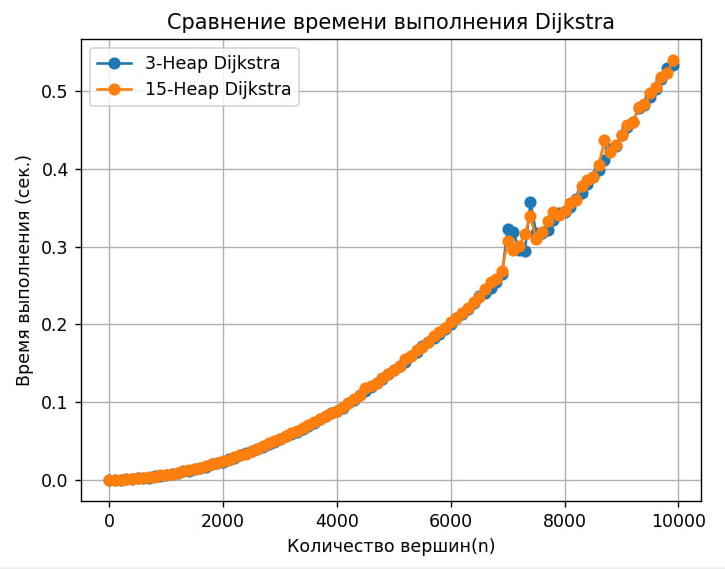
\includegraphics[width=0.8\linewidth]{picture/vertices.png}
    \caption{Сравнение времени выполнения в зависимости от количества вершин}
    \label{fig:vertices}
\end{figure}

На графике~\ref{fig:vertices} представлена зависимость времени выполнения от количества вершин \( n \). Здесь видно, что использование как 3-кучи, так и 15-кучи приводит к схожим результатам. Различия в скорости выполнения становятся заметны только при больших значениях \( n \), при этом 15-куча начинает слегка уступать 3-куче по скорости выполнения. Это может быть связано с тем, что при увеличении арности увеличивается количество операций управления в более крупных кучах.

\begin{figure}[H]
    \centering
    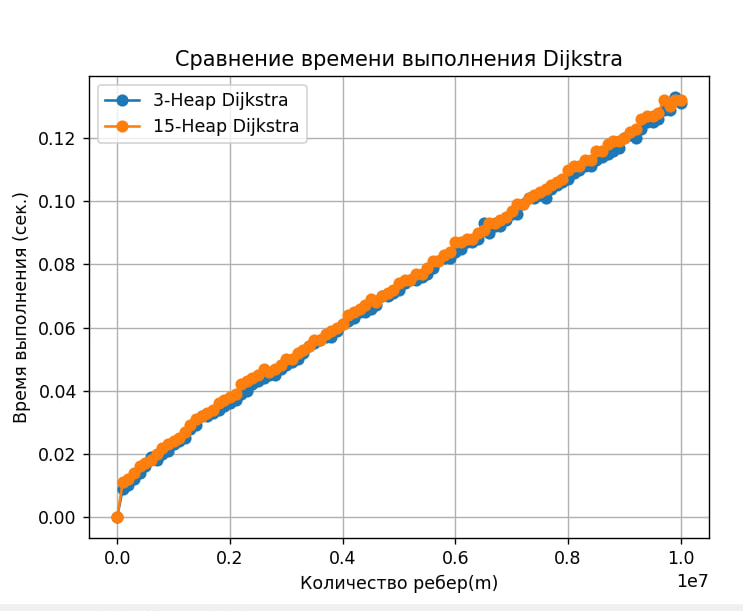
\includegraphics[width=0.8\linewidth]{picture/edges.png}
    \caption{Сравнение времени выполнения в зависимости от количества рёбер}
    \label{fig:edges}
\end{figure}

На графике ~\ref{fig:edges} представлена зависимость времени выполнения от количества рёбер \( m \). В этом случае время выполнения алгоритма также линейно возрастает с увеличением \( m \), и различия между 3-кучей и 15-кучей остаются минимальными. Однако, как и в случае с увеличением вершин, можно заметить, что 15-куча начинает показывать слегка большее время выполнения на больших значениях \( m \). Это связано с тем, что на больших графах операции в 15-куче могут требовать больше времени для поддержания структуры кучи при добавлении и удалении элементов.


\section*{Возможные причины отклонений:}
На графиках также можно заметить незначительные отклонения, которые могут быть обусловлены фоновыми процессами операционной системы, влиянием кэширования и доступом к оперативной памяти. Эти факторы могли вызвать незначительные колебания во времени выполнения, особенно при многократном запуске алгоритма на больших графах.

	\section*{Заключение}
\addcontentsline{toc}{section}{Заключение}
Lorem ipsum dolor sit amet, consectetur adipiscing elit, sed do eiusmod tempor incididunt ut labore et dolore magna aliqua. Ut enim ad minim veniam, quis nostrud exercitation ullamco laboris nisi ut aliquip ex ea commodo consequat. Duis aute irure dolor in reprehenderit in voluptate velit esse cillum dolore eu fugiat nulla pariatur. Excepteur sint occaecat cupidatat non proident, sunt in culpa qui officia deserunt mollit anim id est laborum.

Во время проведения исследования были достигнуты следующие цели и выполнены соответствующие задачи:
\begin{enumerate}
	\item Наберите здесь свой текст.
	\item Наберите здесь свой текст. 
	\item Наберите здесь свой текст.
\end{enumerate}

Полученные результаты исследования позволяют\ldots

В заключение можно отметить\ldots

Таким образом\ldots
    \begin{thebibliography}{99}
	\addcontentsline{toc}{section}{Список литературы}
	\bibitem{Dijkstra}
	Алгоритм Дейкстры // Википедия: свободная энциклопедия. \\ 
	URL: \url{https://en.wikipedia.org/wiki/Dijkstra%27s_algorithm}. 

	\bibitem{Cormen}
	Кормен Т.Х., Лейзерсон Ч.E., Ривест Р.L., Штайн К. Алгоритмы: Построение и анализ / Т.Х. Кормен, Ч.E. Лейзерсон, Р.L. Ривест, К. Штайн. --- 3-е изд. --- М.: Вильямс, 2011.

	\bibitem{Skiena}
	Скиен С. Алгоритмы. Руководство по разработке / С. Скиен. --- М.: Вильямс, 2006. --- 800 с.: ил. ISBN 978-5-8459-0805-7.
\end{thebibliography}

    \section*{Приложение A}\label{prog1}
\addcontentsline{toc}{section}{Приложение A}
\subsection*{Точный алгоритм}
\subsubsection*{main.cpp}
%\lstinputlisting[language=C++]{code/main3.txt}

    
\end{document}